\documentclass[12pt,a4paper]{article}
\usepackage[T1]{fontenc}
\usepackage[utf8]{inputenc}
\usepackage[brazil]{babel}
\usepackage{lmodern}
\usepackage[left=3cm,right=2cm,top=3cm,bottom=2cm]{geometry}
\usepackage{setspace,graphicx,booktabs,array,tabularx,longtable,amsmath,amssymb,needspace}
\usepackage{caption}
\usepackage{xurl}
\usepackage[hidelinks,unicode]{hyperref}
\urlstyle{same}
\hypersetup{pdftitle={Detecção de erros em telemetria sob ruído real},
pdfauthor={Enzo Aurélio; Luís Fernando; Vinicius Campos},pdfsubject={Trabalho prático de Transmissão e Comunicação de Dados}}
\setlength{\parindent}{1.25cm}
\setlength{\parskip}{0.15em}
\setlength{\emergencystretch}{2em}
\clubpenalty=10000
\widowpenalty=10000
\displaywidowpenalty=10000
\renewcommand{\arraystretch}{1.2}
\captionsetup{font=small,labelfont=bf}
\onehalfspacing
\begin{document}
\hypersetup{pageanchor=false}
\begin{titlepage}
\centering
{\large IFMT - OCTAYDE\par}
{\large Transmissão e Comunicação de Dados\par}
\vspace{2.4cm}
{\large Enzo Aurélio\par}
{\large Luís Fernando\par}
{\large Vinicius Campos\par}
\vspace{2.7cm}
{\LARGE\bfseries Detecção de erros em telemetria sob ruído real\par}
\vspace{0.7cm}
{\Large Enlace UART com três ESP32: comparação entre SUM8 e CRC-8\par}
\vspace{1.8cm}
\begin{flushright}
\begin{minipage}{0.62\textwidth}
\singlespacing
Relatório de trabalho prático apresentado à disciplina de Transmissão e Comunicação de Dados.\\[0.5em]
Professor: Ruy Oliveira.
\end{minipage}
\end{flushright}
\vfill
\end{titlepage}
\pagenumbering{roman}
\hypersetup{pageanchor=true}


\section*{Resumo}\addcontentsline{toc}{section}{Resumo}

Este trabalho compara a soma modular de oito bits (SUM8) e o CRC-8/SMBUS em um enlace UART com três ESP32: transmissor, receptor e injetor de ruído físico. O sorteio dos alvos de ruído alcança LEN, sequência, payload e CHK, cobrindo os 64 bits do corpo do quadro. Sete rodadas válidas de 1.000 quadros totalizaram 7.000 posições experimentais e 56.000 amostras do injetor. SUM8 apresentou dois erros não detectados no modo 2, com taxa de 2/621 = 0,3221\% entre os erros checados dessa condição. CRC8 apresentou zero casos não detectados nas três rodadas ensaiadas. Os tempos médios de verificação no RX foram 1,006 \ensuremath{\mu}s e 3,003 \ensuremath{\mu}s, respectivamente. Em controle separado, o RX permaneceu sem recepção por 350,443 ms e voltou a aceitar um quadro 38,691 ms depois de reativar a UART. As conclusões se restringem ao modelo de perturbação ensaiado e distinguem checagem, entrega à aplicação e auditoria posterior.\par

\par\noindent\textbf{Palavras-chave:} ESP32; UART; soma modular; CRC8; ruído físico; telemetria.\par

\clearpage\tableofcontents\clearpage\pagenumbering{arabic}

\section{Introdução e objetivos}

O trabalho compara SUM8 e CRC-8 no mesmo enlace UART. Os códigos, a especificação e os registros estão disponíveis em \url{https://github.com/enzogomes2006/esp32-deteccao-erros-telemetria}. O payload contém quatro bytes sintéticos, não medições de um sensor. Cada condição usa uma técnica por vez. A série física atual foi coletada em 19/10/2026 após sete testes curtos de dez quadros. Dois controles adicionais de dez quadros registraram os tempos de cálculo do TX.\par

Foram avaliadas sete condições de transmissão com o mesmo formato de quadro e a mesma temporização. As observações consideradas nas tabelas pertencem exclusivamente às sete coletas de mil quadros identificadas no Apêndice A. O objetivo é medir a incidência de erros detectados, erros não detectados e falhas de enquadramento, além do custo de cálculo e do tempo de recuperação do receptor.\par

No grupo, Enzo Aurélio ficou responsável pelo transmissor (TX), Vinicius Campos pelo receptor (RX) e Luís Fernando pelo injetor de ruído.\par

\section{Bancada e modelo de ruído}

Três ESP32 clássicos WROOM exercem os papéis TX, RX e RUÍDO. A configuração documentada dos programas é ESP32 Dev Module, CPU de 240 MHz e Arduino-ESP32 3.3.12. A montagem usa GND comum, dois resistores de 1 k\ensuremath{\Omega} e um BC547. TX usa GPIO17, RX usa GPIO16; o injetor observa a linha limpa em GPIO16, a perturbada em GPIO18 e comanda a base pelo resistor em GPIO19. O esquema funcional da Figura \ref{fig:circuito} representa a ligação entre os dispositivos. O mapa detalhado dos fios está documentado no repositório.\par


\begin{figure}[htbp]
\centering
\setlength{\unitlength}{1mm}
\begin{picture}(150,65)
\put(0,40){\framebox(28,14){\shortstack{TX\\GPIO17}}}
\put(28,47){\line(1,0){15}}
\put(43,44){\framebox(23,6){R1: 1 k$\Omega$}}
\put(66,47){\line(1,0){53}}
\put(119,40){\framebox(30,14){\shortstack{RX\\GPIO16}}}
\put(35,47){\circle*{1.3}}
\put(88,47){\circle*{1.3}}
\put(20,58){\makebox(36,4){\small RUÍDO GPIO16}}
\put(72,58){\makebox(40,4){\small RUÍDO GPIO18}}
\put(88,47){\line(0,-1){17}}
\put(76,18){\framebox(24,12){BC547}}
\put(0,17){\framebox(29,14){\shortstack{RUÍDO\\GPIO19}}}
\put(29,24){\line(1,0){14}}
\put(43,21){\framebox(23,6){R2: 1 k$\Omega$}}
\put(66,24){\line(1,0){10}}
\put(88,18){\line(0,-1){11}}
\put(82,7){\line(1,0){12}}
\put(84,5){\line(1,0){8}}
\put(86,3){\line(1,0){4}}
\put(94,4){\makebox(40,5)[l]{\small GND comum}}
\end{picture}
\caption{Ligação funcional do injetor. GPIO16 do RUÍDO observa a linha limpa; GPIO18 observa o ponto do RX. GPIO19 aciona a base pelo resistor R2. O emissor do BC547 e as três placas compartilham GND.}
\label{fig:circuito}
\end{figure}


Na montagem, as maiores dificuldades foram ajustar a injeção de ruído e organizar os cabos de forma que as ligações entre as placas ficassem visíveis e claras.\par

\subsection{Temporização e efeito físico do ruído}

O modo é selecionado pelo Monitor Serial. Ao reconhecer o marcador, o injetor sorteia os alvos e acompanha o início de cada byte na linha limpa. A captura do periférico MCPWM fornece uma referência de tempo de hardware para a borda inicial; a rotina de interrupção consulta esse contador e comanda GPIO19 nos instantes dos bits selecionados. O MCPWM é usado como relógio, sem gerar uma portadora PWM na linha de dados.\par

A 115200 baud, o período de bit é $T_b=1/115200\approx 8{,}68\,\mu\mathrm{s}$. O código reserva margem nominal de $1\,\mu\mathrm{s}$ em cada borda do intervalo selecionado. Um alvo isolado resulta em uma janela nominal de aproximadamente $6{,}68\,\mu\mathrm{s}$; em alvos consecutivos, o transistor permanece acionado ao longo da região contígua. Os pulsos preservam os bits de start e stop.\par

O injetor força a linha ao nível baixo em instantes selecionados. Um alvo em bit já zero não muda o byte. O log separa máscara selecionada de máscara efetivamente alterada e registra os oito bytes antes/depois, sincronismo e atrasos. Os resultados dependem da captura e amostragem dessa bancada; a revisão lógica dos registros não substitui uma medição de forma de onda ou calibração elétrica independente.\par

\begin{table}[htbp]\centering\small\caption{Modos de seleção dos alvos de ruído.}\begin{tabular}{>{\raggedright\arraybackslash}p{\dimexpr 0.300\linewidth-2\tabcolsep\relax}>{\raggedright\arraybackslash}p{\dimexpr 0.700\linewidth-2\tabcolsep\relax}}\toprule

\textbf{Modo} & \textbf{Seleção de alvos no corpo} \\

\midrule

0 & Sem pulsos de ruído \\

1 & Uma posição entre os 64 bits \\

2 & Duas posições distintas entre os 64 bits \\

3 & Rajada contígua de 3 a 8 bits em um dos oito bytes \\

4 & Controle extra nos bits 7 de P0 e P1; fora das sete rodadas \\

\bottomrule\end{tabular}\end{table}

O marcador e a referência de depuração são preservados. Os ensaios não cobrem corrupção deliberada do marcador nem dos bits UART de start/stop. A rajada do modo 3 fica dentro de um byte, conforme o sorteio implementado.\par

\section{Protocolo serial e detectores}

O enlace é UART 115200 baud, 8N1, unidirecional, sem ACK nem retransmissão. O quadro tem doze bytes:\par

\begin{quote}\begin{minipage}{\linewidth}\begin{singlespace}\small\begin{verbatim}
A5 5A C3 3C | 07 seqL seqH p0 p1 p2 p3 CHK
\end{verbatim}\end{singlespace}\end{minipage}\end{quote}

\begin{table}[htbp]\centering\small\caption{Campos do quadro de dados transmitido.}\begin{tabular}{>{\raggedright\arraybackslash}p{\dimexpr 0.200\linewidth-2\tabcolsep\relax}>{\raggedright\arraybackslash}p{\dimexpr 0.120\linewidth-2\tabcolsep\relax}>{\raggedright\arraybackslash}p{\dimexpr 0.680\linewidth-2\tabcolsep\relax}}\toprule

\textbf{Campo} & \textbf{Bytes} & \textbf{Regra} \\

\midrule

Marcador & 4 & A5 5A C3 3C; fora da checagem \\

LEN & 1 & 07; sete bytes posteriores a LEN \\

Sequência & 2 & uint16 little-endian \\

Payload & 4 & Telemetria sintética; bits 7 de P0/P1 fixados em 1 \\

CHK & 1 & SUM8 ou CRC8, conforme a rodada \\

\bottomrule\end{tabular}\end{table}

O RX reconhece o marcador, coleta oito bytes de corpo e exige LEN=7. Um LEN alterado não aumenta o limite de leitura. Se LEN for inválido, o quadro não chega à checagem e é classificado PERDIDO por enquadramento. O parser volta à busca de marcadores. Um marcador dentro do corpo é tratado como dado.\par

\subsection{SUM8}

O TX calcula CHK = -soma(LEN, seqL, seqH, p0, p1, p2, p3) módulo 256. O RX soma os oito bytes, incluindo CHK. Resíduo diferente de zero implica descarte. Alterações cuja diferença total seja múltipla de 256 mantêm o resíduo zero e podem produzir aceitação indevida.\par

\begin{align}c&=\left(-\sum_{i=0}^{6}d_i\right)\bmod 256,\\r&=\left(\sum_{i=0}^{7}d_i\right)\bmod 256.\end{align}

\subsection{CRC-8/SMBUS}

O programa representa o polinômio gerador por 0x07, omitindo o termo de grau oito. Os parâmetros são init=0, refin=false, refout=false e xorout=0. O TX calcula sobre sete bytes; o RX processa os oito e espera resíduo zero. O cálculo percorre cada byte MSB primeiro, enquanto a UART transmite seus bits LSB primeiro. O teste padrão da implementação é CRC8 de "123456789" = F4.\par

\begin{equation}G(x)=x^8+x^2+x+1.\end{equation}

O CRC calcula um resto polinomial em GF(2), com XOR. A ausência de erros não detectados nas rodadas CRC8 não constitui garantia de detecção de qualquer padrão de corrupção. LEN inválido é tratado pelo enquadramento antes da verificação de qualquer detector.\par

\subsection{Decisão, enlace e referência}

Após o quadro, o TX envia D5 6A B4 4B seguido de uma cópia dos oito bytes originais. A linha DECISAO\_ANTES\_DA\_COPIA documenta a decisão antes da leitura da referência. A cópia serve para auditar e associar a posição experimental; não corrige o payload entregue nem o estado da sequência do enlace.\par

Corpos descartados não têm sequência confiável. O RX mantém eventos anônimos até conciliá-los com uma sequência aceita, sem transformar cada descarte em uma segunda perda. Sequências antigas ou repetidas não geram nova entrega. seq\_rx conserva o que chegou, e seq\_referencia/seq\_experimento identificam a auditoria posterior. cabecalho\_diverge registra divergências de LEN ou sequência, inclusive se um detector aceitar. ACEITO pelo detector e entregue\_aplicacao são campos distintos.\par

O RX espera no máximo 60 ms pelo bloco ou pela auditoria. Para ausência de progresso de dados, o prazo é 250 ms, com avanço de 100 ms por ausência adicional. O primeiro marcador inicia o controle de ausência; novos marcadores e decisões de dados renovam o prazo. A referência não o renova. Antes do primeiro marcador, o RX apenas aguarda o início da transmissão. Referência ausente, órfã, inválida ou associação ambígua invalida a medição.\par

O intervalo medido entre quadros tem mediana de 101 ms e máximo de 101,917 ms nas sete séries. Assim, $250/101\approx2{,}48$: o prazo de ausência tolera mais de dois períodos antes de registrar uma falta. O passo de 100 ms acompanha o período nominal do TX. Para o quadro e sua cópia, os 24 bytes em UART 8N1 levam nominalmente $240/115200\approx2{,}08$ ms, além de 44 ms de pausas programadas. O limite de 60 ms supera esses 46,08 ms nominais e deixa margem de processamento, sem manter o RX esperando indefinidamente. Os prazos são atendidos pelo loop; não são medições de disparo exato de um timer.\par

\section{Método e conferência dos dados}

Foram selecionadas quatro condições SUM8, modos 0 a 3, e três CRC8, modos 1 a 3, com mil quadros cada. O controle sem ruído CRC8 foi registrado entre os controles curtos, sem substituir nenhuma das sete condições. Cada pasta conserva os CSVs do RX e do injetor, os logs brutos, os metadados e a revisão automática. Somente as sete condições de mil quadros entram nas tabelas principais; os controles de temporização e recuperação são analisados separadamente.\par

A conferência recalculou contagens e resíduos, cruzou os oito bytes com as amostras do injetor e verificou máscaras, efeito físico, sincronismo, atrasos, identidade das posições e ordem de decisão/auditoria. Os CSVs foram comparados com os logs brutos. O validador publicado em coletor/Revisar.ps1 permite repetir a revisão dos registros. As tabelas usam registros coletados nas placas, não as saídas dos testes de software.\par

\begin{table}[htbp]\centering\small\caption{Critérios de classificação dos quadros.}\begin{tabular}{>{\raggedright\arraybackslash}p{\dimexpr 0.300\linewidth-2\tabcolsep\relax}>{\raggedright\arraybackslash}p{\dimexpr 0.700\linewidth-2\tabcolsep\relax}}\toprule

\textbf{Classe} & \textbf{Critério experimental} \\

\midrule

OK & Checagem aceitou e payload coincide com referência válida \\

CORROMPIDO & Checagem concluída; resíduo diferente de zero \\

PERDIDO & Sem checagem concluída: enquadramento ou ausência evidenciada \\

NAO\_DETECTADO & Checagem aceitou, mas payload difere da referência válida \\

\bottomrule\end{tabular}\end{table}

Cada posição recebe uma única classe. A taxa de não detecção considera os quadros com erro efetivo em que a checagem foi concluída. OK e PERDIDO ficam fora desse denominador. Quando não há erro checado, a taxa é n.a., não zero por convenção. Um alvo já zero não constitui erro real. Contagens de condições diferentes não são amostras pareadas do mesmo ruído.\par

\begin{equation}\text{Taxa ND}=\frac{N_{\mathrm{ND}}}{N_{\mathrm{CORROMPIDO}}+N_{\mathrm{ND}}}.\end{equation}

\section{Resultados das sete rodadas}

\begin{table}[htbp]\centering\small\caption{Resultados SUM8: mil quadros por modo.}\label{tab:sum8}
\begin{tabular}{lrrrrr}\toprule
Modo & OK & Corrompido & Perdido & Não detectado & Taxa ND \\
\midrule
0 & 1000 & 0 & 0 & 0 & n.a. \\
1 & 563 & 392 & 45 & 0 & 0,0000\% \\
2 & 289 & 619 & 90 & 2 & 0,3221\% \\
3 & 100 & 809 & 91 & 0 & 0,0000\% \\
\bottomrule\end{tabular}\end{table}

\begin{table}[htbp]\centering\small\caption{Resultados CRC8: mil quadros por modo.}\label{tab:crc8}
\begin{tabular}{lrrrrr}\toprule
Modo & OK & Corrompido & Perdido & Não detectado & Taxa ND \\
\midrule
1 & 540 & 418 & 42 & 0 & 0,0000\% \\
2 & 305 & 593 & 102 & 0 & 0,0000\% \\
3 & 116 & 792 & 92 & 0 & 0,0000\% \\
\bottomrule\end{tabular}\end{table}

Cada linha soma 1.000 posições; cada rodada tem 8.000 amostras do injetor e rodada\_valida=SIM. A conferência encontrou zero cabeçalhos divergentes em corpos aceitos nas sete rodadas. Divergências em corpos descartados ou malformados permanecem nos registros.\par

\begin{figure}[htbp]\centering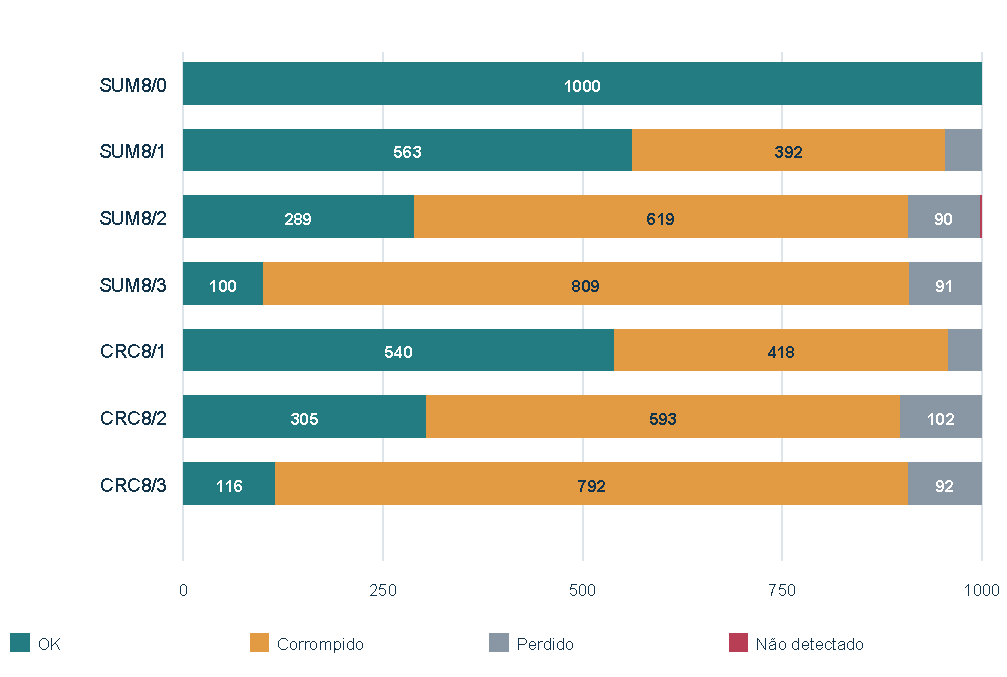
\includegraphics[width=\linewidth]{figuras/contagens.pdf}\caption{Classes registradas por condição, com mil quadros em cada barra. Os dois ND do SUM8/2 são identificados na tabela e no estudo de caso; sua largura é pequena nessa escala.}\end{figure}

\subsection{Taxas e perdas de enquadramento}



Na rodada SUM8/2 ocorreram 621 erros checados, sendo 619 detectados e 2 não detectados. A taxa é 0,3221\%. Em relação aos mil quadros transmitidos, os dois casos são 0,2\%; esse é outro denominador e não substitui a taxa definida. Os 90 perdidos são excluídos da taxa de falha do detector.\par

Todas as perdas registradas nas sete condições tiveram motivo LEN\_INVALIDO. Portanto, nesta série PERDIDO representa falha de enquadramento observada, e não comprova desaparecimento completo do quadro. A ampliação do ruído ao cabeçalho explica por que a CORPO64 contém perdas mesmo com os marcadores preservados. O ensaio de recepção desligada é apresentado separadamente.\par

\subsection{Dois casos naturais não detectados}

As sequências 415 e 553 da rodada SUM8/2 foram aceitas e entregues à aplicação com payload errado. Em ambos os casos, o log do injetor confirma alteração de 1 para 0 nos dois alvos, sincronismo SIM e ausência de flags de amostragem ou pulso tardio.\par

\begin{table}[htbp]\centering\small\caption{Bytes efetivamente alterados nos dois casos não detectados.}\begin{tabular}{>{\raggedright\arraybackslash}p{\dimexpr 0.200\linewidth-2\tabcolsep\relax}>{\raggedright\arraybackslash}p{\dimexpr 0.200\linewidth-2\tabcolsep\relax}>{\raggedright\arraybackslash}p{\dimexpr 0.200\linewidth-2\tabcolsep\relax}>{\raggedright\arraybackslash}p{\dimexpr 0.200\linewidth-2\tabcolsep\relax}>{\raggedright\arraybackslash}p{\dimexpr 0.200\linewidth-2\tabcolsep\relax}}\toprule

\textbf{Sequência} & \textbf{Campo} & \textbf{Transmitido} & \textbf{Recebido} & \textbf{Máscara real} \\

\midrule

415 & P0 & 87 & 07 & 80 \\

415 & CHK & E7 & 67 & 80 \\

553 & P3 & B3 & 33 & 80 \\

553 & CHK & 89 & 09 & 80 \\

\bottomrule\end{tabular}\end{table}

Todos os valores de bytes e máscaras nessa tabela são hexadecimais. Os corpos completos são:\par

\begin{quote}\begin{minipage}{\linewidth}\begin{singlespace}\small\begin{verbatim}
seq 415 TX: 07 9F 01 87 BA 1E 13 E7
seq 415 RX: 07 9F 01 07 BA 1E 13 67
seq 553 TX: 07 29 02 EA CF D9 B3 89
seq 553 RX: 07 29 02 EA CF D9 33 09
\end{verbatim}\end{singlespace}\end{minipage}\end{quote}

Na sequência 415, a soma dos oito bytes transmitidos é 768, e a soma recebida é 512. Na sequência 553, as somas são 1.024 e 768. Os cálculos completos são apresentados abaixo. Apagar dois bits 7 reduz a soma em 128+128=256. Os dois valores de cada par continuam múltiplos de 256; o detector mantém resíduo zero. Em cada caso LEN e sequência permanecem intactos, enquanto payload e CHK mudam. A colisão foi observada em ruído aleatório do modo 2, sem usar o controle extra do modo 4.\par

\begin{align*}
S_{415,TX}&=7+159+1+135+186+30+19+231=768,\\
S_{415,RX}&=7+159+1+7+186+30+19+103=512,\\
S_{553,TX}&=7+41+2+234+207+217+179+137=1024,\\
S_{553,RX}&=7+41+2+234+207+217+51+9=768.
\end{align*}
Em ambos os casos, a diferença é $-256$ e o resto da soma recebida módulo 256 continua zero.\par

\begin{table}[htbp]\centering\small\caption{Extrato do log do injetor nos dois casos não detectados. Bytes e máscaras em hexadecimal; horários do próprio injetor.}\begin{tabular}{lrrrrrr}\toprule Sequência & Campo & Antes & Depois & Alvo & Mudou & Instante ($\mu$s)\\\midrule

415 & P0 & 87 & 07 & 80 & 80 & 811647755 \\

415 & CHK & E7 & 67 & 80 & 80 & 811659755 \\

553 & P3 & B3 & 33 & 80 & 80 & 825594709 \\

553 & CHK & 89 & 09 & 80 & 80 & 825597709 \\

\bottomrule\end{tabular}\label{tab:log-injetor}\end{table}

O evento 416, correspondente à sequência 415, decide ACEITO em 709748318 \ensuremath{\mu}s e só depois registra referência em 709762509 \ensuremath{\mu}s. O evento 554, sequência 553, decide em 723686327 \ensuremath{\mu}s e recebe referência em 723700531 \ensuremath{\mu}s. Esses pares pertencem ao relógio do RX. Os timestamps absolutos do injetor não foram subtraídos dos timestamps do RX.\par

\section{Tempos, taxa e overhead}

\subsection{Cálculo no transmissor}

Controles separados de dez quadros, sem ruído, registraram 1 \ensuremath{\mu}s por cálculo SUM8 e 3 \ensuremath{\mu}s por cálculo CRC8. Em cada técnica, os nove intervalos após o primeiro quadro foram 101000 \ensuremath{\mu}s, ou 101 ms. O primeiro intervalo zero foi excluído. Os corpos transmitidos foram comparados com as referências das respectivas coletas curtas e coincidem. Os registros estão em evidencias/.\par

\subsection{Verificação no receptor}

\begin{table}[htbp]\centering\small\caption{Tempo de verificação dos quadros no receptor.}\begin{tabular}{>{\raggedright\arraybackslash}p{\dimexpr 0.140\linewidth-2\tabcolsep\relax}>{\raggedright\arraybackslash}p{\dimexpr 0.140\linewidth-2\tabcolsep\relax}>{\raggedright\arraybackslash}p{\dimexpr 0.230\linewidth-2\tabcolsep\relax}>{\raggedright\arraybackslash}p{\dimexpr 0.230\linewidth-2\tabcolsep\relax}>{\raggedright\arraybackslash}p{\dimexpr 0.130\linewidth-2\tabcolsep\relax}>{\raggedright\arraybackslash}p{\dimexpr 0.130\linewidth-2\tabcolsep\relax}}\toprule

\textbf{Condição} & \textbf{N checados} & \textbf{Média (\ensuremath{\mu}s)} & \textbf{Mediana (\ensuremath{\mu}s)} & \textbf{Mín.} & \textbf{Máx.} \\

\midrule

SUM8/0 & 1000 & 1,011 & 1,0 & 1 & 2 \\

SUM8/1 & 955 & 1,009 & 1,0 & 1 & 7 \\

SUM8/2 & 910 & 1,002 & 1,0 & 1 & 2 \\

SUM8/3 & 909 & 1,002 & 1,0 & 1 & 2 \\

CRC8/1 & 958 & 3,005 & 3,0 & 3 & 5 \\

CRC8/2 & 898 & 3,002 & 3,0 & 3 & 4 \\

CRC8/3 & 908 & 3,002 & 3,0 & 3 & 4 \\

\bottomrule\end{tabular}\end{table}

Os corpos com LEN inválido não chegaram à checagem e têm tempo NA. Foram excluídos das estatísticas de verificação, sem substituir ausência por zero. A média agregada SUM8 usa 3.774 checagens e vale 1,006 \ensuremath{\mu}s. CRC8 usa 2.764 checagens e vale 3,003 \ensuremath{\mu}s. Essas médias são ponderadas pelas amostras individuais, e não médias simples das linhas da tabela.\par

\begin{figure}[htbp]\centering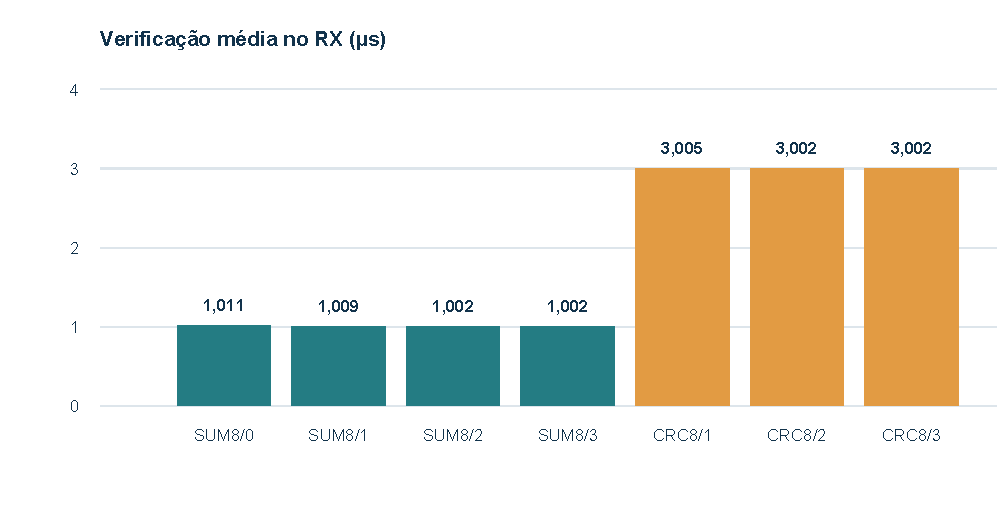
\includegraphics[width=\linewidth]{figuras/tempos_rx.pdf}\caption{Média de verificação do RX nas sete condições. Unidade: microssegundos. Os tamanhos amostrais estão na tabela. A resolução registrada é de microssegundos; o log e o processamento da bancada podem afetar os extremos.}\end{figure}

\subsection{Intervalos e custo de transmissão}

\begin{table}[htbp]\centering\small\caption{Intervalos entre inícios de quadros, medidos pelo RX.}\begin{tabular}{>{\raggedright\arraybackslash}p{\dimexpr 0.200\linewidth-2\tabcolsep\relax}>{\raggedright\arraybackslash}p{\dimexpr 0.200\linewidth-2\tabcolsep\relax}>{\raggedright\arraybackslash}p{\dimexpr 0.200\linewidth-2\tabcolsep\relax}>{\raggedright\arraybackslash}p{\dimexpr 0.200\linewidth-2\tabcolsep\relax}>{\raggedright\arraybackslash}p{\dimexpr 0.200\linewidth-2\tabcolsep\relax}}\toprule

\textbf{Condição} & \textbf{N intervalos} & \textbf{Média (ms)} & \textbf{Mín. (ms)} & \textbf{Máx. (ms)} \\

\midrule

SUM8/0 & 999 & 101,001 & 100,998 & 101,917 \\

SUM8/1 & 999 & 101,000 & 100,992 & 101,023 \\

SUM8/2 & 999 & 101,001 & 100,998 & 101,917 \\

SUM8/3 & 999 & 101,001 & 100,998 & 101,917 \\

CRC8/1 & 999 & 101,001 & 100,998 & 101,917 \\

CRC8/2 & 999 & 101,000 & 101,000 & 101,023 \\

CRC8/3 & 999 & 101,000 & 100,999 & 101,023 \\

\bottomrule\end{tabular}\end{table}

Os intervalos são medidos pelo RX entre inícios de quadros e usam 999 diferenças por rodada. A mediana é 101 ms em todas as condições. Não são tempos de recuperação nem incluem o primeiro zero.\par

Cada quadro de dados tem 4 bytes úteis e 8 de overhead: marcador 4, LEN 1, sequência 2 e CHK 1. A eficiência em bytes é 4/12=33,33\%; overhead/total=66,67\% e overhead/payload=200\%. A cópia de depuração fica fora dessa conta de overhead, como determina o enunciado.\par

Em 8N1, cada byte ocupa dez bits na linha. Os 12 bytes de dados ocupam teoricamente 120/115200 s, cerca de 1,042 ms. Esses valores não incluem as pausas programadas de 10 ms após o marcador, 3 ms por byte do corpo e 10 ms antes da referência. O período observado de 101 ms resulta de todo o agendamento, não de uma mudança na taxa UART. Com quatro bytes úteis a cada 101 ms, a vazão útil aproximada é 39,60 bytes/s, ou 316,83 bit/s.\par

\section{Recuperação após interrupção de recepção}

O controle SUM8 de dez quadros usa ruído configurado em zero e desliga a UART do RX após auditar a sequência 1. É uma interrupção programada da recepção, sem alterar o firmware entre cálculo e recuperação. Os eventos e horários foram extraídos do registro rx\_recuperacao\_SUM8\_10.log, preservado em evidencias/. O registro foi consolidado sem duplicar as linhas da região de sobreposição entre os trechos disponíveis. Não há captura complementar do monitor do injetor para esse controle.\par

\begin{table}[htbp]\centering\small\caption{Instantes do controle de recuperação registrados pelo RX.}\begin{tabular}{>{\raggedright\arraybackslash}p{\dimexpr 0.300\linewidth-2\tabcolsep\relax}>{\raggedright\arraybackslash}p{\dimexpr 0.700\linewidth-2\tabcolsep\relax}}\toprule

\textbf{Evento do RX} & \textbf{Instante (\ensuremath{\mu}s)} \\

\midrule

RX\_DESLIGADO & 94561283 \\

Primeira detecção de ausência & 94797303 \\

RX\_REATIVADO & 94911726 \\

Aceitação da sequência 5 & 94950417 \\

\bottomrule\end{tabular}\end{table}

A janela efetiva sem recepção foi 94911726-94561283=350443 \ensuremath{\mu}s, ou 350,443 ms. O tempo da reativação até a primeira aceitação foi 94950417-94911726=38691 \ensuremath{\mu}s, ou 38,691 ms. Desde a primeira detecção de perda até a aceitação foram 153114 \ensuremath{\mu}s, ou 153,114 ms. As medidas têm origens diferentes e não devem receber o mesmo rótulo.\par

O resumo registra 7 OK, 3 PERDIDOS (sequências 2, 3 e 4), zero CORROMPIDOS e zero ND. As sete auditorias somadas às três ausências evidenciadas contabilizam dez posições. O RX informa rodada\_valida=SIM, zero ambiguidades e sequência esperada final 10. As perdas não são preenchidas com referências inventadas. Esse controle não entra nas sete condições de ruído.\par

\section{Discussão e limites}

Os dois casos SUM8 demonstram uma limitação concreta da soma modular: alterações no payload e no próprio detector podem preservar o resto. O CRC8 não apresentou ND nos modos ensaiados. As diferenças de OK entre técnicas também dependem dos sorteios e dos valores dos bytes; as rodadas não reutilizaram exatamente o mesmo ruído, portanto a diferença bruta de contagens não mede isoladamente uma vantagem do algoritmo.\par

A cópia posterior torna a auditoria possível, mas integra a instrumentação experimental. O resultado OK da tabela é definido pelo payload; divergências de cabeçalho precisam ser avaliadas nos campos específicos. A observação de zero cabeçalhos aceitos divergentes nesta série não elimina a possibilidade de colisões futuras no cabeçalho.\par

A ordenação uint16 e a passagem de 65535 para zero foram verificadas em software, mas as rodadas físicas de 0 a 999 não exercitam esse cruzamento. As mensagens de versão foram observadas durante a gravação; não houve leitura de flash nem verificação criptográfica do binário instalado. As mensagens de versão identificam a execução observada, mas não equivalem a uma leitura do binário instalado.\par

\Needspace{13\baselineskip}

\section{Conclusão}

A revisão CORPO64 produziu sete séries físicas consistentes e ampliou os alvos de ruído aos oito bytes do corpo. Dois payloads incorretos passaram pelo SUM8 no modo 2 e foram entregues, com evidência byte a byte e resíduo zero. O CRC8 registrou zero ND nas três condições ensaiadas. A verificação custou aproximadamente 1 \ensuremath{\mu}s no SUM8 e 3 \ensuremath{\mu}s no CRC8, muito abaixo do período de 101 ms adotado na bancada. O controle separado mostrou retomada após uma pausa de recepção, com distinção entre tempo sem UART, tempo após reativação e tempo desde a detecção de perda. Os dados e o validador permitem conferir a consolidação, dentro dos limites instrumentais descritos.\par

\clearpage\appendix\section{Rastreabilidade e reprodução}

\begin{table}[htbp]\centering\small\caption{Pastas das sete séries experimentais.}\begin{tabular}{>{\raggedright\arraybackslash}p{\dimexpr 0.300\linewidth-2\tabcolsep\relax}>{\raggedright\arraybackslash}p{\dimexpr 0.700\linewidth-2\tabcolsep\relax}}\toprule

\textbf{Condição} & \textbf{Pasta original em dados/} \\

\midrule

SUM8/0 & 20261019\_091242\_692\_SUM8\_modo0\_1000 \\

SUM8/1 & 20261019\_094547\_976\_SUM8\_modo1\_1000 \\

SUM8/2 & 20261019\_095219\_782\_SUM8\_modo2\_1000 \\

SUM8/3 & 20261019\_095929\_835\_SUM8\_modo3\_1000 \\

CRC8/1 & 20261019\_100416\_161\_CRC8\_modo1\_1000 \\

CRC8/2 & 20261019\_100921\_806\_CRC8\_modo2\_1000 \\

CRC8/3 & 20261019\_101329\_766\_CRC8\_modo3\_1000 \\

\bottomrule\end{tabular}\end{table}

Cada pasta contém seis arquivos originais. Os metadados identificam a configuração da rodada e revisao.txt registra a conferência do coletor. A revisão pode ser repetida pelo coletor, usando os logs brutos. O repositório reúne os programas, a especificação do protocolo e os registros necessários para conferir as contagens e os casos discutidos.\par

Para repetir a revisão de uma coleta no Windows, executar na raiz do repositório, substituindo o nome da pasta para conferir as outras seis séries:\par

\begin{quote}\begin{minipage}{\linewidth}\begin{singlespace}\small\begin{verbatim}
powershell.exe -NoProfile -ExecutionPolicy Bypass `
  -File coletor/Coletor.ps1 `
  -ReviewFolder dados/20261019_091242_692_SUM8_modo0_1000
\end{verbatim}\end{singlespace}\end{minipage}\end{quote}

\clearpage
\begin{thebibliography}{9}
\addcontentsline{toc}{section}{Referências}
\bibitem{enunciado} IFMT. \textit{Trabalho prático: detecção de erro em telemetria sob ruído real (ESP32)}. Material da disciplina de Transmissão e Comunicação de Dados.
\bibitem{repositorio} Enzo Aurélio; Luís Fernando; Vinicius Campos. \textit{Detecção de erros em telemetria com ESP32: códigos e registros experimentais}. 2026. Disponível em: \url{https://github.com/enzogomes2006/esp32-deteccao-erros-telemetria}. Acesso em: 19 out. 2026.
\end{thebibliography}
\end{document}
